% --------------------------------------------
\documentclass{Arquivos/AcademicoPadrao} 
% --------------------------------------------
% Dados Pré-Textuais
% --------------------------------------------
\titulo{Relatório Técnico:\\ {\large Modelo Conforme Normas UFT/ABNT}}

\autor{\WenesTex Aquino}

\orientador{\WenesTex Gomes Aquino}
\coorientador{Beltrano Vitória Almeida}

\local{Arraias -- TO}
\data{2025, v-2.0}

\instituicao{%
  Universidade Federal do Tocantins \\
  Campus Universitário de Palmas \\
  Curso de Licenciatura em Computação
}


\tipotrabalho{Trabalho de Conclusão de Curso}


\preambulo{Relatório Técnico apresentado como 
    parte dos requisitos para avaliação na Universidade 
    Federal do Tocantins. Este modelo foi adaptado 
    e personalizado com ajustes visuais e estruturais, 
    servindo também para testar o espaço disponível 
    utilizada nessa contracapa. Por \WenesTex.}




\begin{document}
\nocite{*}


\pretextual % =================================


\folhaderosto
\contracapa


% ======== RELATÓRIO e TCC ==========%
\capituloCentralizado*{Agradecimentos}
Elemento opcional. Devem ser inseridos após a errata, se houver.




% ======== RELATÓRIO e TCC ==========%
\begin{resumo}
Este resumo está em conformidade com a \textbf{ABNT NBR 6028:2021}, que estabelece os requisitos para a redação e apresentação de resumos, resenhas e recensões. O resumo é definido como a apresentação concisa dos pontos relevantes de um documento. O texto deve ser composto por uma sequência de \textbf{frases concisas em parágrafo único}, sem enumeração de tópicos. Para trabalhos acadêmicos e relatórios técnicos, como este, recomenda-se a modalidade informativa e a extensão de 150 a 500 palavras. Convém que o texto seja redigido utilizando o \textbf{verbo na terceira pessoa}. As \textbf{palavras-chave} devem figurar logo abaixo do resumo, antecedidas da expressão "Palavras-chave:", \textbf{separadas entre si por ponto e vírgula (;)} e \textbf{finalizadas por ponto (.)}.

\textbf{Palavras-chaves}: \WenesTex; ABNT NBR 6028:2021; resumo informativo; parágrafo único; ponto e vírgula; relatório técnico.
\end{resumo}


\begin{resumoEN}

\end{resumoEN}


\listaDeFiguras
\listaDeTabelas


\begin{siglas}
    \item[CPU] Unidade Central de Processamento
    \item[RAM] Memória de Acesso Aleatório
    \item[SSD] Unidade de Estado Sólido (Solid State Drive)
\end{siglas}


\begin{simbolos}
    \item[$\alpha$] Alfa (Ângulo, Coeficiente de Temperatura)
    \item[$\beta$] Beta (Ângulo, Ganho de Corrente do Transistor)
    \item[$\sum$] Somatório (Usado em Séries Matemáticas e Estatística)
\end{simbolos}

\Sumario


\textual % ==================================


\capituloCentralizado{Introdução}


\part{Preparação} % Opcional
\chapter{Desenvolvimento}
\section{Estrutura do relatório}

{\SingleSpacing
\[
\begin{aligned}
\text{Parte externa} &=
\begin{cases}
\quad\text{Capa (opcional)}\\
\quad\text{Lombada (opcional)}
\end{cases}
\\[3em]
\text{Parte interna} &=
\begin{cases}
\text{Elementos pré-textuais} &
\begin{cases}
\quad\text{Folha de rosto (obrigatório)}\\
\quad\text{Errata (opcional)}\\
\quad\text{Agradecimentos (opcional)}\\
\quad\text{Resumo na língua vernácula (obrigatório)}\\
\quad\text{Lista de ilustrações (opcional)}\\
\quad\text{Lista de tabelas (opcional)}\\
\quad\text{Lista de abreviaturas e siglas (opcional)}\\
\quad\text{Lista de símbolos (opcional)}\\
\quad\text{Sumário (obrigatório)}
\end{cases}
\\\rule{0pt}{4em}
\text{Elementos textuais} &
\begin{cases}
\quad\text{Introdução (obrigatório)}\\
\quad\text{Desenvolvimento (obrigatório)}\\
\quad\text{Considerações finais (obrigatório)}
\end{cases}
\\\rule{0pt}{7em}
\text{Elementos pós-textuais} &
\begin{cases}
\quad\text{Referências (obrigatório)}\\
\quad\text{Glossário (opcional)}\\
\quad\text{Apêndice (opcional)}\\
\quad\text{Anexo (opcional)}\\
\quad\text{Índice (opcional)}\\
\quad\text{Formulário de identificação (opcional)}
\end{cases}
\end{cases}
\end{aligned}
\]}


\part{Resultado} % Opcional
\chapter{Considerações finais}
\section{Conclusão}


\postextual % ==================================


\capituloCentralizado{Referências}
\printbibliography[heading=none]


\paginaDivisoria{APÊNDICES}
\inicioApendices
\chapter{Apêndice}


\paginaDivisoria{ANEXOS}
\inicioAnexos
\chapter{Identificado Maiúsculas consecutivas Respectivo Título}
\section{Nulla malesuada porttitor diam}
\lipsum[3-10]
\subsection{Pellentesque habitant morbi}
\lipsum[8-15]

\begin{table}[ht]
    \centering
    \caption{Tabela estilosa 5×5}
    \label{tab:estilosa}
    \begin{tabular}{ccccc}
        \toprule
        Col 1 & Col 2 & Col 3 & Col 4 & Col 5 \\
        \midrule
        A1 & B1 & C1 & D1 & E1 \\
        A2 & B2 & C2 & D2 & E2 \\
        A3 & B3 & C3 & D3 & E3 \\
        A4 & B4 & C4 & D4 & E4 \\
        A5 & B5 & C5 & D5 & E5 \\
        \bottomrule
    \end{tabular}
\end{table}

\begin{figure}[ht]
    \centering
    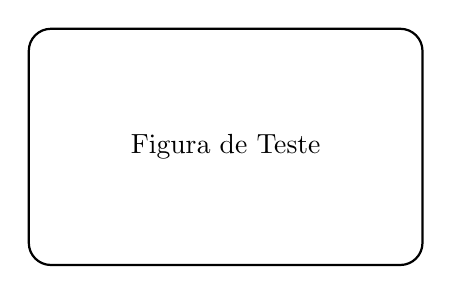
\begin{tikzpicture}
        \draw[rounded corners=8pt, thick] (0,0) rectangle (5,3);
        \node at (2.5,1.5) {Figura de Teste};
    \end{tikzpicture}
    \caption{Figura de teste estilizada}
    \label{fig:teste-estilosa}
\end{figure}

\end{document} 